\documentclass[a4paper]{article}

\usepackage{amsmath}
\usepackage{amsthm}
\usepackage{amssymb}
\usepackage{parskip}
\usepackage[backend=bibtex]{biblatex}
\usepackage{makecell}
\usepackage{adjustbox}
\usepackage[hang]{subfigure}
\usepackage{dirtree}

\usepackage{lpi}
\usepackage{tikz-uml}

\usetikzlibrary{lindenmayersystems}
\usetikzlibrary[shadings]
\usetikzlibrary{
	cd % tikz-cd communitative diagrams
}

\addbibresource{./references.bib}
\graphicspath{ {./media} }

\title{%
    Lindenmayer's Garden \\
    \phantom{} \\
    \Large Scuola d'Arti e Mestieri di Trevano (SAMT) \\
    \Large Documentation
}

\author{Paolo Bettelini}

\date{}

\lpisetup%
    {Lindenmayer's Garden}

\newtheorem{theorem1}{Theorem}
\renewcommand\qedsymbol{$\blacksquare$}

\makenoidxglossaries

\newglossaryentry{GUI}
{
    name=GUI,
    description={Graphical User Interface.
    A type of user interface that allows users to interact
    with a computer program using graphical elements}
}

\newglossaryentry{trait}
{
    name=trait,
    description={A trait in Rust defines shared behavior among structures}
}

\newglossaryentry{cargo}
{
    name=cargo,
    description={Package manager for the Rust programming language}
}

\newglossaryentry{Rust}
{
    name=Rust,
    description={A systems programming language
    designed for speed, safety, and concurrency,
    which is known for its memory safety and thread safety features}
}

\newglossaryentry{C}
{
    name=C,
    description={A general-purpose computer programming language}
}

\newglossaryentry{C++}
{
    name=C++,
    description={An object-oriented programming language derived from C}
}

\newglossaryentry{CSS}
{
    name=CSS,
    description={Cascading Style Sheets.
    a stylesheet language used to describe the look
    and formatting of HTML documents}
}

\newglossaryentry{CAS}
{
    name=CAS,
    description={Computer Algebra System}
}

\newglossaryentry{GTK}
{
    name=GTK,
    description={GIMP Toolkit}
}

\newglossaryentry{Gantt}
{
    name=Gantt,
    description={A bar chart that illustrates a project schedule}
}

\newglossaryentry{waterfall}
{
    name=waterfall,
    description={classical model used in system development life cycle to create a system with a linear and sequential approach}
}


\begin{document}

\maketitle

%-F++F-
\pgfdeclarelindenmayersystem{A}{
  \symbol{S}{\pgflsystemstep=0.625\pgflsystemstep}
  \rule{F->-F++F-}
}

\vspace{4.5cm}

\begin{center}
    \begin{tikzpicture}[]
        \draw
        [blue!50!black,thin,line cap=round]
        l-system [l-system={A,axiom=F
        ,order=10,angle=45,step=0.2cm}];
    \end{tikzpicture}
\end{center}

\pagebreak

\begin{center}
    \thispagestyle{empty}
    \vspace*{\fill}
    \textsl{I would like to thank my professor Geo Petrini for this amazing project.}
    \vspace*{\fill}
\end{center}

\pagebreak

\tableofcontents

\pagebreak

\section{Introduction}

\subsection{Abstract}

Lindenmayer Systems, or commonly L-systems,
are formal grammars used for generating complex patterns and structures.
They were introduced in 1968 by Aristid Lindenmayer, a Hungarian theoretical biologist and botanist.
These systems are exceptionally good at representing natural growth of trees, algae, bushes and such.
L-systems can also be used to draw any sort of fractal, with a variable level of detail.
The goal of this project is to stimulate creativity
by creating a L-system playground.
The program provides a sophisticated deterministic context-free grammar
with advanced drawing features, stochastic behavior and an animation system. \\
Furthermore, L-systems are Turing-complete, meaning that anything can be computed
with them.
Any geometrical shape can be mathematically modelled with these systems. \\
There are many programs that can be used to render L-systems, but none of them
approaches the topic the same way this project is intended to.
The philosophy behind this implementation is to let the user experiment
with arbitrary mathematical expressions, and be as flexible as possible.

\subsection{Information}

This is a project of the Scuola Arti e Mestieri di Trevano (SAMT) under the following circumstances

\begin{itemize}
    \item \textbf{Section}: Computer Science
    \item \textbf{Year:} Fourth
    \item \textbf{Class:} LPI
    \item \textbf{Supervisor:} Geo Petrini
    \item \textbf{Expert:} Gionata Genazzi
    \item \textbf{Title:} Lindenmayer's Garden
    \item \textbf{Start date}: 2023-05-02
    \item \textbf{Deadline}: 2023-05-26
\end{itemize}

and the following requirements

\begin{itemize}
    \item \textbf{Documentation}: a full documentation of the work done
    \item \textbf{Diary}: constant changelog for each working session
    \item \textbf{Source code}: source code of the project
\end{itemize}

All the source code and documents can be found at
\href{http://gitsam.cpt.local/lavoro\_finale\_lpi\_2023/giardino-lindenmayer}
{http://gitsam.cpt.local/lavoro\_finale\_lpi\_2023/giardino-lindenmayer}
\cite{gitrepo}.

\pagebreak

\section{L-systems}

\subsection{Formal grammar}

In theory of computation and formal language theory, a formal grammar\cite{formalgrammar} is a system
describing a language of a given alphabet using a set of production rules.

\subsection{Context-free grammar}

A context-free grammar\cite{contextfreegrammar}
is a formal grammar where the production rules for a given symbol are always the same.
For each symbol, the production rule for that symbol is independent of the other symbols
in the string or any other external factor.

\subsection{Fractals}

A fractal\cite{fractal} is a geometrical shape that is self-similar
and contains an arbitrary large amount of detail.

\subsection{Definition}

An \textit{L-system}\cite{lsystem} or \textit{Lindenmayer system}
is a type of formal grammar which can be used to
draw fractals and other shapes. \\
The grammar of an L-system may vary.
The language of such systems may be generated using grammars such as context-free grammars,
stochastic grammars, sensitive grammars and many more.

An L-system may be expressed as a tuple
\(G=(\Sigma, \omega, P)\)
where \(\Sigma\) is the alphabet, \(\omega \in \Sigma^*\) is the
\textit{initial string}, \textit{axiom} or
\textit{initiator} and \(P \subseteq \Sigma \times \Sigma^*\) is a set of production rules.

Any L-system can produce a string by applying its productions
rules \(P\) to every symbol of a string.
Let this operation be defined as \(\pi:P\times \Sigma^* \to \Sigma^*\).
The result of \(\pi(P, v)\) will be a copy of \(v\),
but if \(\exists\, (a,b) \in P \,|\, v \text{ contains } a\), then the symbol \(a\)
in \(v\) will be replaced by the string \(b\).

In general, this operation can be applied iteratively starting with the axiom \(\omega\).
\begin{align*}
    G_0 &= \omega \\
    G_1 &= \pi(P, \omega) \\
    G_2 &= \pi(P, \pi(P, \omega)) \\
    G_3 &= \pi(P, \pi(P, \pi(P, \omega))) \\
    \vdots \\
    G_n &= \pi(P, G_{n-1})
\end{align*}
where \(n\in \mathbb{N}\) is the number of iterations.

\subsection{Semantics}

In order to give meaning to \(v \in \Sigma^*\)
I first define my own structure, \(W\), which is an extension of a classical
L-system \(G=(\Sigma, \omega, P)\). \\
The language of \(W\) is generated using a deterministic context-free grammar,
but the semantics can behave in a stochastic manner.

\(W\) is a tuple \((G, V, O, c)\)
where \(V = {\mathbb{R}^k}\) is a tuple of \textit{variables},
\(O\) is a set of \textit{operations},
and \(c\) is a tuple of \textit{configurations}.

% Definition of I
The set \(I\) is defined as \(I=\mathbb{N} \times \Sigma^*\).

% Definition of c
\pagebreak
The tuple \(c\) contains the following values:
\begin{enumerate}
    \item \texttt{iter} \(\in \mathbb{N}\).
    \item \texttt{initial rotation} \(\in [0; 2\pi]\).
    \item \texttt{initial position} \(\in {\mathbb{R}}^2\).
    \item \texttt{initial thickness} \(\in \mathbb{R}\).
    \item \texttt{initial color} \(\in {\mathbb{R}}^4\).
    \item \texttt{background color} \(\in {\mathbb{R}}^4\).
    \item \texttt{canvas} \(\in {\mathbb{R}}^2\).
    %\item \texttt{seed} \(\in \mathbb{Z}\).
    \item \texttt{injections} \(\in I^n\).
\end{enumerate}

% Definition of Expression
Let \(\text{Expr}\) be an algebraic data type\cite{adt}
representing any mathematical expression, including stochastic functions.

% Definition of Xi
Let \(\Xi_S\) be an algebraic data type defined as
\begin{align*}
    \Xi_S =\,
    &\text{Forward}(\text{Expr})\,&|\quad
    &\text{Jump}(\text{Expr})\,&|\quad
    &\text{Dot}(\text{Expr})\,&| \\
    &\text{Rotate}(\text{Expr})\,&|\quad
    &\text{Thickness}(\text{Expr})\,&|\quad
    &\text{Color}(\mathbb{R}^4)\,&| \\
    &\text{Ignore}(\text{Expr})\,&|\quad
    &\text{Push}()\,&|\quad
    &\text{Pop}()\,&| \\
    &\text{Update}(\mathbb{N}, \text{Expr})\,&
\end{align*}
This data type is based and acts on a mutable globally shared state \(S\).
There exists a function \(\text{eval} : \Xi_S \to \mathbb{R}\)
that evaluates the value of \(\Xi_S\). \\
Any Expr type may use variables in the state \(S\).
The state \(S\) initially contains every variable in \(V\).
The evaluation of \(\Xi_S \equiv \text{Update}(i, j)\)
will update the value \(i\)-th value of \(V\) in \(S\) to \(\text{eval}(j)\). \\
\(S\) also acts as a stack data structure. Whenever \(\Xi_S \equiv \text{Pop}()\),
the state of \(S\) becomes the state last of \(S\) before the last instance where
\(\Xi_S \equiv \text{Push}()\). \\
Every other constructor of \(\Xi_S\), except for \(\Xi_S \equiv \text{Ignore}(j)\),
has a graphical meaning.

% Definition of O
The set \(O\) is defined \(O \subseteq \Sigma \times \mathcal{P}([\Xi])\)
where \([\Xi]\) denotes all possible values for \(\Xi\).

%%%% Functions

% inject
Let \(\phi : I \times \Sigma^* \to \Sigma^*\) be the \texttt{inject} function.
The function \(\phi(i, v)\) where \(i=(\gamma, \zeta)\)
will construct a string by injecting the string \(\zeta\)
at the position \(\gamma\) of the string \(v\) if \(\gamma \leq |v|\).

% multi inject
Let \(\Phi: I^n \times \Sigma^* \to \Sigma^*\)
be the \texttt{multi-inject} function.
The function \(\Phi(\Psi, v)\) will construct the string \(v_n\),
starting from \(v_0 = v\), by applying \(v_i = \phi(\psi, v_{i-1})\)
for all values \(\psi\) in \(\Psi\) considering the order in \(\Psi\).

% ignore
Let \(\theta : \mathbb{N} \times \mathbb{N} \times \Sigma^* \to \Sigma^*\)
be the \texttt{ignore} function.
The function \(\theta(i, l, v)\) will construct a string that is a copy of \(v\)
but replacing the symbols from the index \(\text{min}(i, |v|)\) to
\(\text{min}(i+l, |v|)\) of \(v\) with the empty string \(\lambda\).

% multi ignore
Let \(\Theta: \Sigma^* \to \Sigma^*\)
be the \texttt{multi-ignore} function.
The function \(\Theta(v)\) will construct a string,
starting from \(v_0 = v\), by applying \(v_i = \theta(i, l, v_{i-1})\)
as long as \(\exists\, (s, o) \in O \,|\, v \text{ contains } s \land
o\equiv \text{Ignore}(j)\) where \(i\) is the position of \(s\) in \(v\)
and \(l=\text{eval}(\text{j})\).

The structure \(W\) can also produce a string \(W_n \in \Sigma^*\)
which is defined as
\[
    W_n = \Theta(\Phi(\text{injections}, G_n))
\]

where \(n\in \mathbb{N}\) is the number of iterations.
The application of \(\text{eval}(v)\, \forall v\in W_\text{iter}\) will produce a graphical drawing.

\pagebreak

\subsection{Turing Completeness of \(W\)}


\begin{theorem1}
    The system \(W=(G, V, O, c)\) is Turing-complete.
\end{theorem1}
    
\begin{proof}
    Since the Lindenmayer system \(G=(\Sigma, \omega, P)\)
    is Turing-complete, we can construct \(W\) such that every \(G_n\)
    can be generated by \(W_n\). \\
    Let \(W=(G, V, O, c)\) where \(V = \emptyset\), \(O = \emptyset\)
    and \texttt{injections}\(\,=\emptyset\).
    \\
    As a corollary, we have:
    \[
        \text{injections} = \emptyset
        \implies \Phi(\text{injections}, v)
        \equiv \Phi(\emptyset, v) \equiv v  
    \]
    and
    \[
        O = \emptyset \implies
        \Theta(v) \equiv v
    \]
    Using this properties, we can simplify the expression for \(W_n\)
    \[
        W_n = \Theta(\Phi(\text{injections}, G_n))
        = G_n
    \]
    Thus, \(W\) is Turing-complete.
\end{proof}

\pagebreak

\subsection{Examples}

The following section shows some examples of L-systems
fractal drawings.

Note that by convention, \texttt{F} means draw a line,
\texttt{+} and \texttt{-} mean rotate by \(\pm \text{angle}\),
\texttt{[} and \texttt{]} mean \texttt{push} and \texttt{pop}
on the stack respectively.

\pgfdeclarelindenmayersystem{Koch curve}{
    \rule{F -> F-F++F-F}
}

\begin{figure}[h]
\begin{minipage}{0.5\textwidth}
    \begin{tikzpicture}
        \pgfset{lindenmayer system/.cd, angle=60, step=2pt}
    
        \pgftransformshift{\pgfqpoint{0cm}{0cm}}
        \pgfpathmoveto{\pgfpointorigin}
        \pgflindenmayersystem{Koch curve}{F++F++F}{4}
        \color{blue!50!black}
        \pgfusepath{stroke}
    
        \pgftransformshift{\pgfqpoint{1.9cm}{1.1cm}}
        \pgfpathmoveto{\pgfpointorigin}
        \pgflindenmayersystem{Koch curve}{F++F++F}{3}
        \color{green!50!black}
        \pgfusepath{stroke}
    
        \pgftransformshift{\pgfqpoint{0.675cm}{0.375cm}}
        \pgfpathmoveto{\pgfpointorigin}
        \pgflindenmayersystem{Koch curve}{F++F++F}{2}
        \color{red!50!black}
        \pgfusepath{stroke}
    \end{tikzpicture}
    \caption{Koch curve for \(n=\) {\color{blue!50!black}4}, {\color{green!50!black}3}, {\color{red!50!black}2}.}
\end{minipage}
\begin{minipage}{0.5\textwidth}
    \(G=(\Sigma, \omega, P)\)
    where
    \begin{itemize}
        \item \(\Sigma = \{'F', '+', '-'\}\)
        \item \(\omega = F++F++F\)
        \item \(P = \{('F', F-F++F-F)\}\)
    \end{itemize}
    and \(\text{angle}=\frac{\pi}{3}\)
\end{minipage}
\end{figure}

\begin{figure}[h]
\begin{minipage}{0.5\textwidth}
    
\begin{tikzpicture}
        \usetikzlibrary {lindenmayersystems}
        \tikz[rotate=65]\draw [green!60!black] l-system
        [l-system={rule set={F -> F[+F]F[-F]}, axiom=F, order=4, angle=25,step=10pt}];
    \end{tikzpicture}
    \caption{Plant for \(n=4\).}
\end{minipage}
\begin{minipage}{0.5\textwidth}
    \(G=(\Sigma, \omega, P)\)
    where
    \begin{itemize}
        \item \(\Sigma = \{'F', '+', '-', '[', ']'\}\)
        \item \(\omega = F\)
        \item \(P = \{('F', F[+F]F[-F])\}\)
    \end{itemize}
    and \(\text{angle}=\frac{5\pi}{36}\)
\end{minipage}
\end{figure}

\pagebreak

\section{Analysis}

\subsection{Requirements}

\requirement{00}{Functionality}{1}{1.0}{none}{
The program must be able to render on a \gls{GUI} any L-system,
within the computational power of the host.
}{}

\requirement{01}{Grammar}{1}{1.0}{none}{
The grammar must support the basic operations of turtle graphics\cite{turtlegraphics}
for D0l-systems.
}{
    \subreq{01}{0}{The grammar must be able to set the color of lines.}
    \subreq{01}{1}{The grammar must be able to set thickness of lines.}
    \subreq{01}{2}{The grammar must be able to ignore the behavior of any given character at any position.}
}

\requirement{02}{Stochastic Behavior}{1}{1.0}{none}{
Variables, such as line lengths or rotation angles, must be able
to follow stochastic behavior.
}{
    \subreq{02}{0}{Stochasic behavior must be based on a deterministic seed.}
}

\requirement{03}{Animations}{2}{1.0}{This implies the use of a variable \texttt{frames} and \texttt{depth}}{
L-systems must be able to support optional animations.
}{
    \subreq{03}{0}{Variables can be dependent on the current animation frame index.}
    \subreq{03}{1}{Variables can be dependent on the current stack depth.}
}

\requirement{04}{Graphical User Interface}{1}{1.0}{none}{
The \gls{GUI} must contain a canvas on which the fractals are rendered.
}{
    \subreq{04}{0}{The \gls{GUI} must provide functionality to modify every rule and aspect of a given L-system.}
    \subreq{04}{1}{The \gls{GUI} must provide functionality to import a file, representing L-systems.}
    \subreq{04}{2}{The GU\gls{GUI}I must provide functionality to export a file, representing L-systems.}
    \subreq{04}{3}{The \gls{GUI} must have an animation playback.}
}

\requirement{05}{Logging}{1}{1.0}{none}{
The program must provide logging capabilities.
}{}

\requirement{06}{Error Checking}{1}{1.0}{none}{
Erroneous input from the user must be handled correctly
with appropriate error messages.
}{
    \subreq{06}{0}{The user must be provided with the information of where he has made a mistake.}
}

\pagebreak

\subsection{Use Cases}

The following diagram shows the use cases of the program.
In order to view a fractal, the user can either import a configuration file
or design a fractal with the graphical editor. \\
When the application starts, an empty configuration is imported by default.
The user may also design his fractal with the editor starting from any configuration.

The user is also able to export the configuration to a file. \\
The fractal itself can be animated.

\begin{center}
\begin{tikzpicture}
    \begin{umlsystem}[x=1] {} % empty title
        \umlusecase[x=1, y=-2, name=vf, width=1.5cm] {View Fractal}

        \umlusecase[x=1, y=1, name=ef, width=2cm] {Export Configuration}
        
        \umlusecase[x=1, y=-6, name=a, width=1.5cm] {Animate}

        \umlusecase[x=6, y=-4.75, name=s, width=1cm] {Stop}
        \umlusecase[x=6, y=-6, name=p, width=1cm] {Play}
        \umlusecase[x=6, y=-7.25, name=r, width=1cm] {Reset}

        \umlusecase[x=6, y=1, name=lc, width=2cm] {Load Configuration}
        \umlusecase[x=6, y=-2, name=dwg, width=2cm] {Design with GUI}
    \end{umlsystem}
    \node [above] at (current bounding box.north) {Application};

    \umlactor[x=-1, y=-2] {User}

    \umlassoc{User}{vf}

    \draw [tikzuml dependency style] (ef) -- node[left] {\(\ll extends \gg\)} (vf);

    \draw [tikzuml dependency style] (a) -- node[left] {\(\ll extends \gg\)} (vf);
    
    \draw [tikzuml dependency style] (r) -- node[below] {\(\ll extends \gg\)} (a);
    \draw [tikzuml dependency style] (s) -- node[above] {\(\ll extends \gg\)} (a);
    \draw [tikzuml dependency style] (p) -- node[above] {\(\ll extends \gg\)} (a);
    
    \draw [tikzuml dependency style] (vf) -- node[right] {\(\ll includes \gg\)} (lc);
    \draw [tikzuml dependency style] (vf) -- node[above] {\(\ll includes \gg\)} (dwg);
\end{tikzpicture}
\end{center}

\pagebreak

\subsection{GUI Design}

The design is very simple and consists of a single page.
The interface has an editor (right side) and a canvas where the image
is displayed. Beneath the canvas is an animation playback to control the animation
system along with some information.

\begin{figure}[h]
    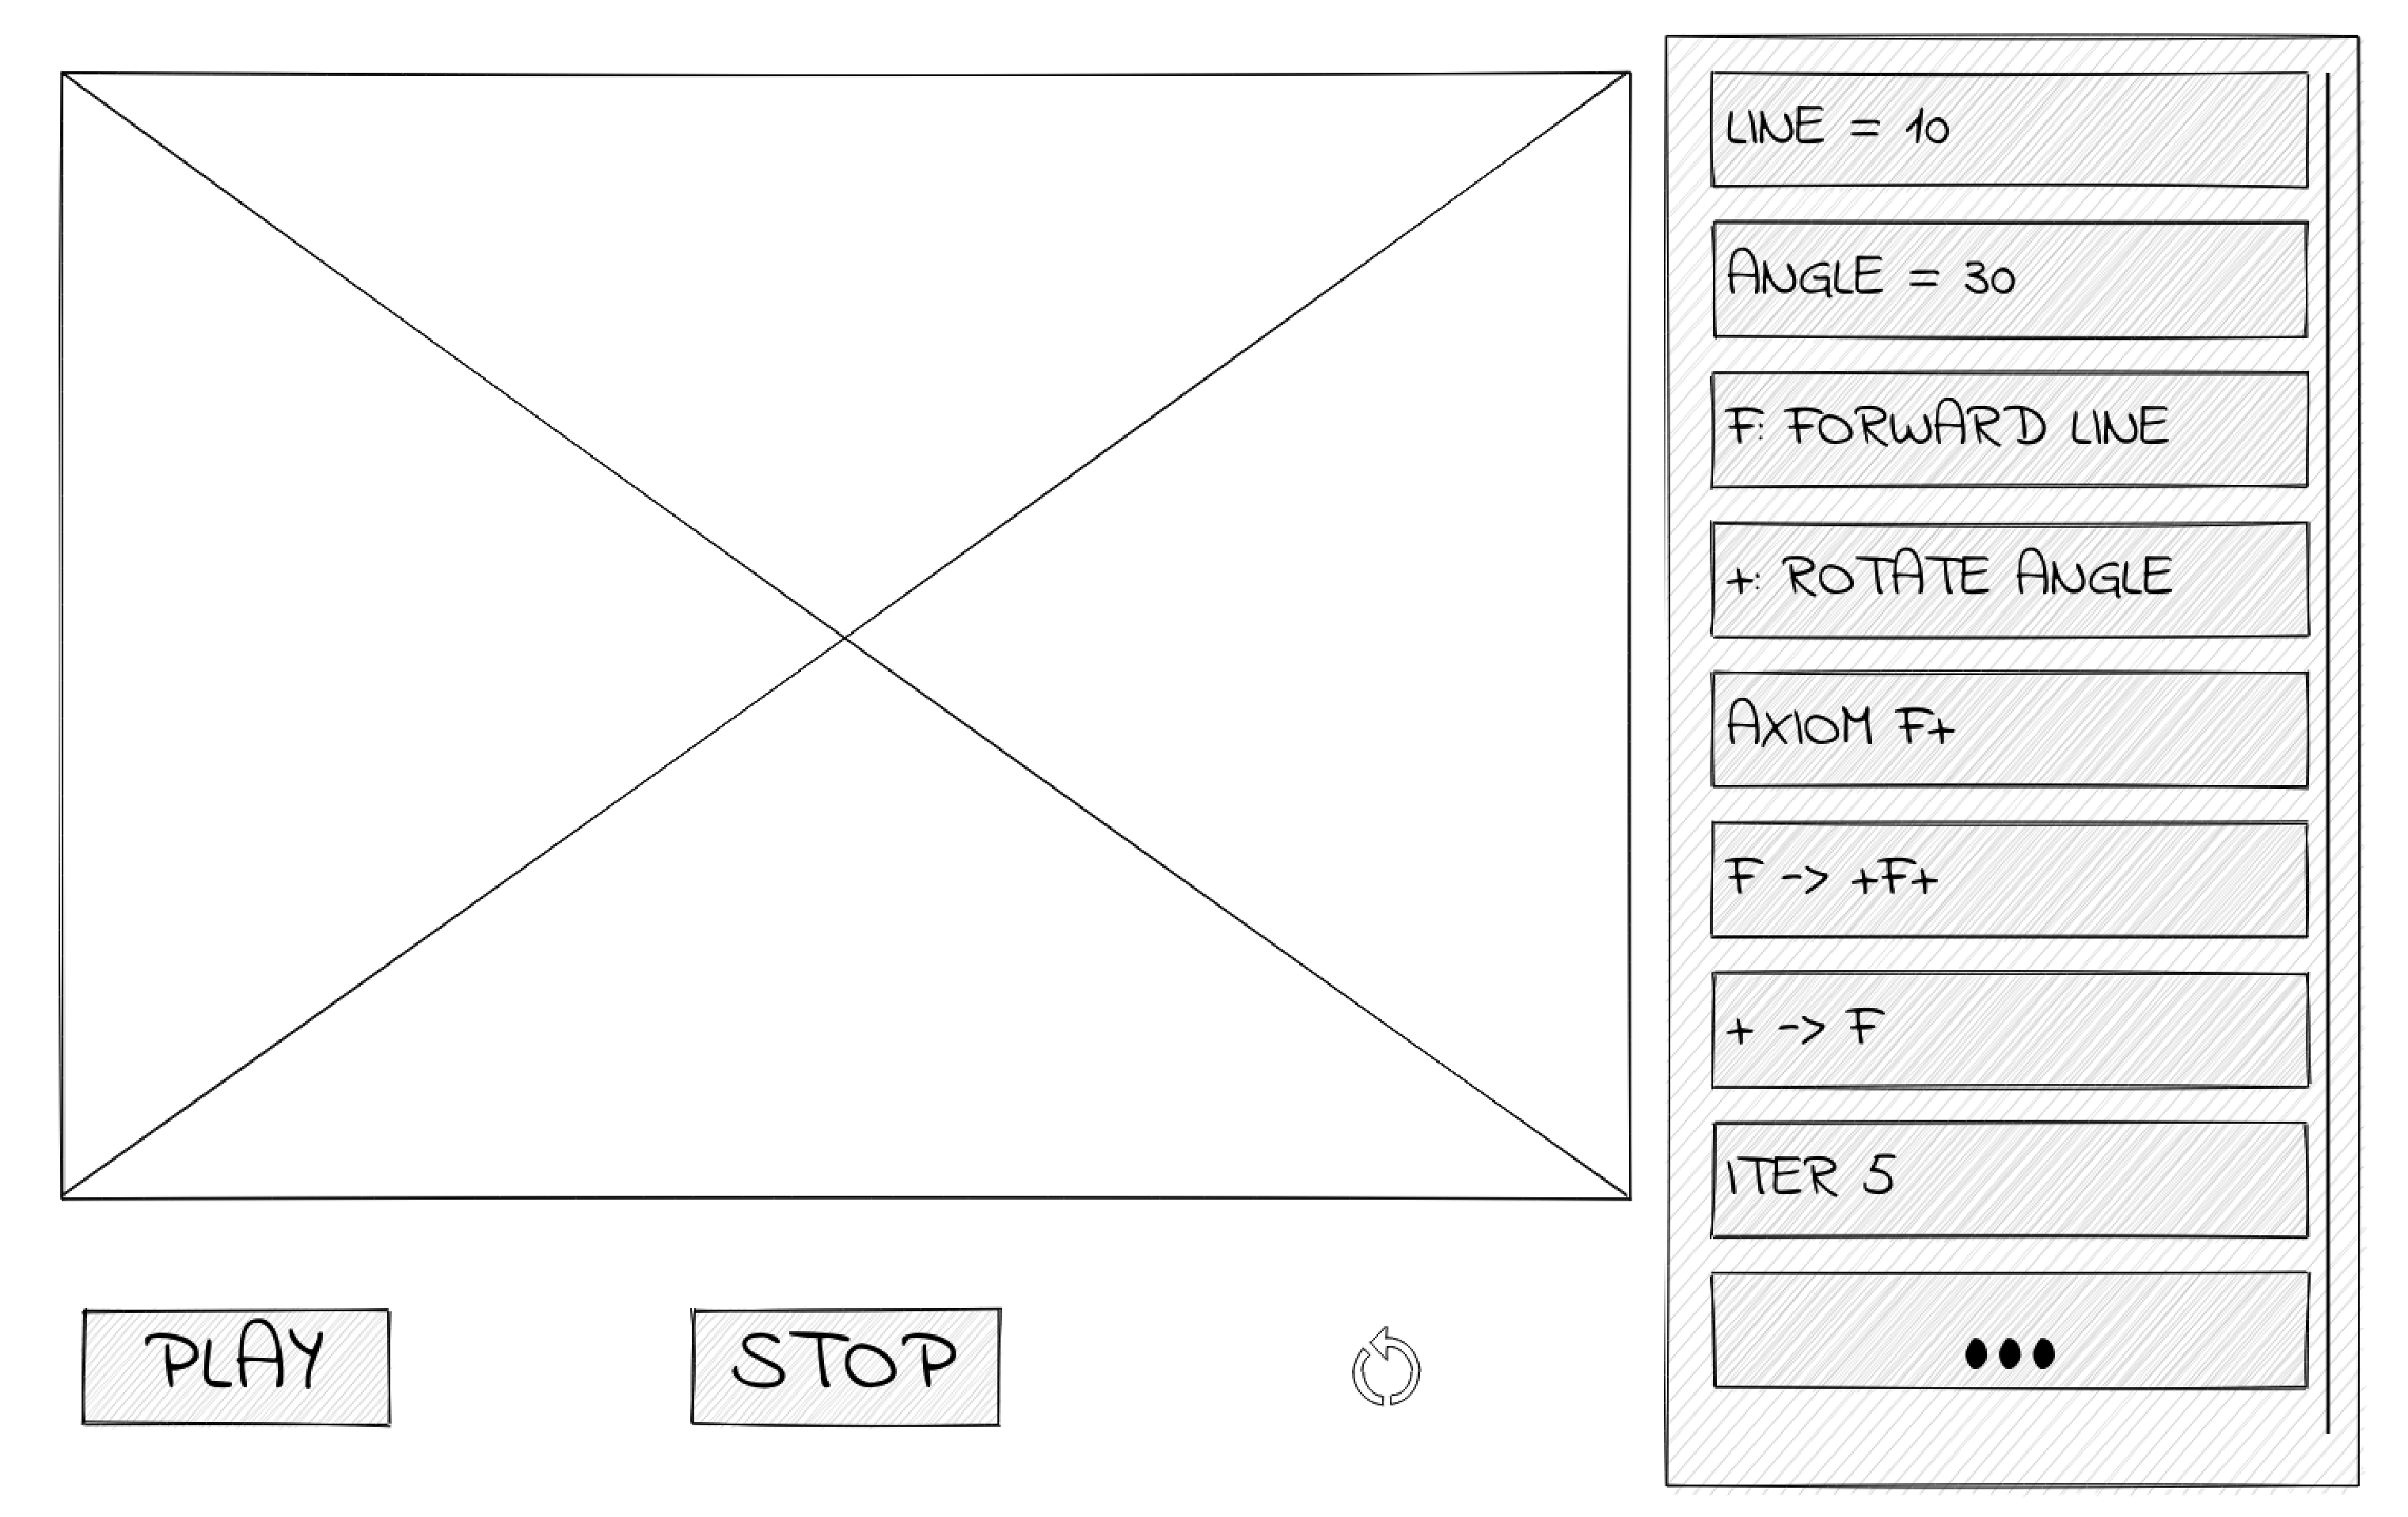
\includegraphics[width=\textwidth]{media/design/ui_design.pdf}
    \caption{GUI Design sketch}
\end{figure}

\pagebreak

\section{Technologies}

\subsection{Rust}

\gls{Rust}\cite{rust} is a generic compiled programming language.
The code is compiled using LLVM to machine code and its speed
is comparable to \gls{C} and \gls{C++}.
\gls{Rust} is the first programming language to guarantee memory safety;
memory is not manually freed nor garbage collected.
It is not possible to dereference a null pointer, cause memory segfauls, %\gls{segfault}s,
core dumps and memory leaks.
Code that could cause undefined behavior can still be written,
but it is strictly bounded in blocks where the compiler is relaxed.
This relaxation implies that the language is also low-level.
Another key feature to the performance of \gls{Rust} is zero cost abstraction,
which means that generic types and function abstractions are resolved at compile-time.
Conditional compilation and compile-time computations are also extensively used.
\\
There are also many features concerning the programming experience, such as
advanced metaprogramming and code generation using macros, intelligent compiler,
dependency system (Cargo), modern syntax and many tools to ease development.

\textbf{\color{red} Note}: a \gls{Rust} \textit{crate} refers to a library.
A \textit{feature} is an optional component of library.
A \textit{module} is a logical section of a program or library.

\subsection{GTK4}

\gls{GTK} (GIMP Toolkit) is a free and open-source widget toolkit for
creating graphical user interfaces (\gls{GUI}s).
\gls{GTK} is written in \gls{C} and has bindings for many programming languages,
including Rust.
\gls{GTK} is widely used in Linux desktop environments and applications,
but it also runs on other platforms, including Windows and macOS.

\gls{GTK}4 was released in December 2020.
It introduces several new features and improvements over its predecessor,
\gls{GTK}3.

\subsection{Cairo}

Cairo\cite{cairo} is a widely used 2D graphics library.
This library is written in C but there exist bindings for almost every language.

\pagebreak

\section{Planning}

\subsection{Initial Gantt Chart}

\begin{figure}[h]
    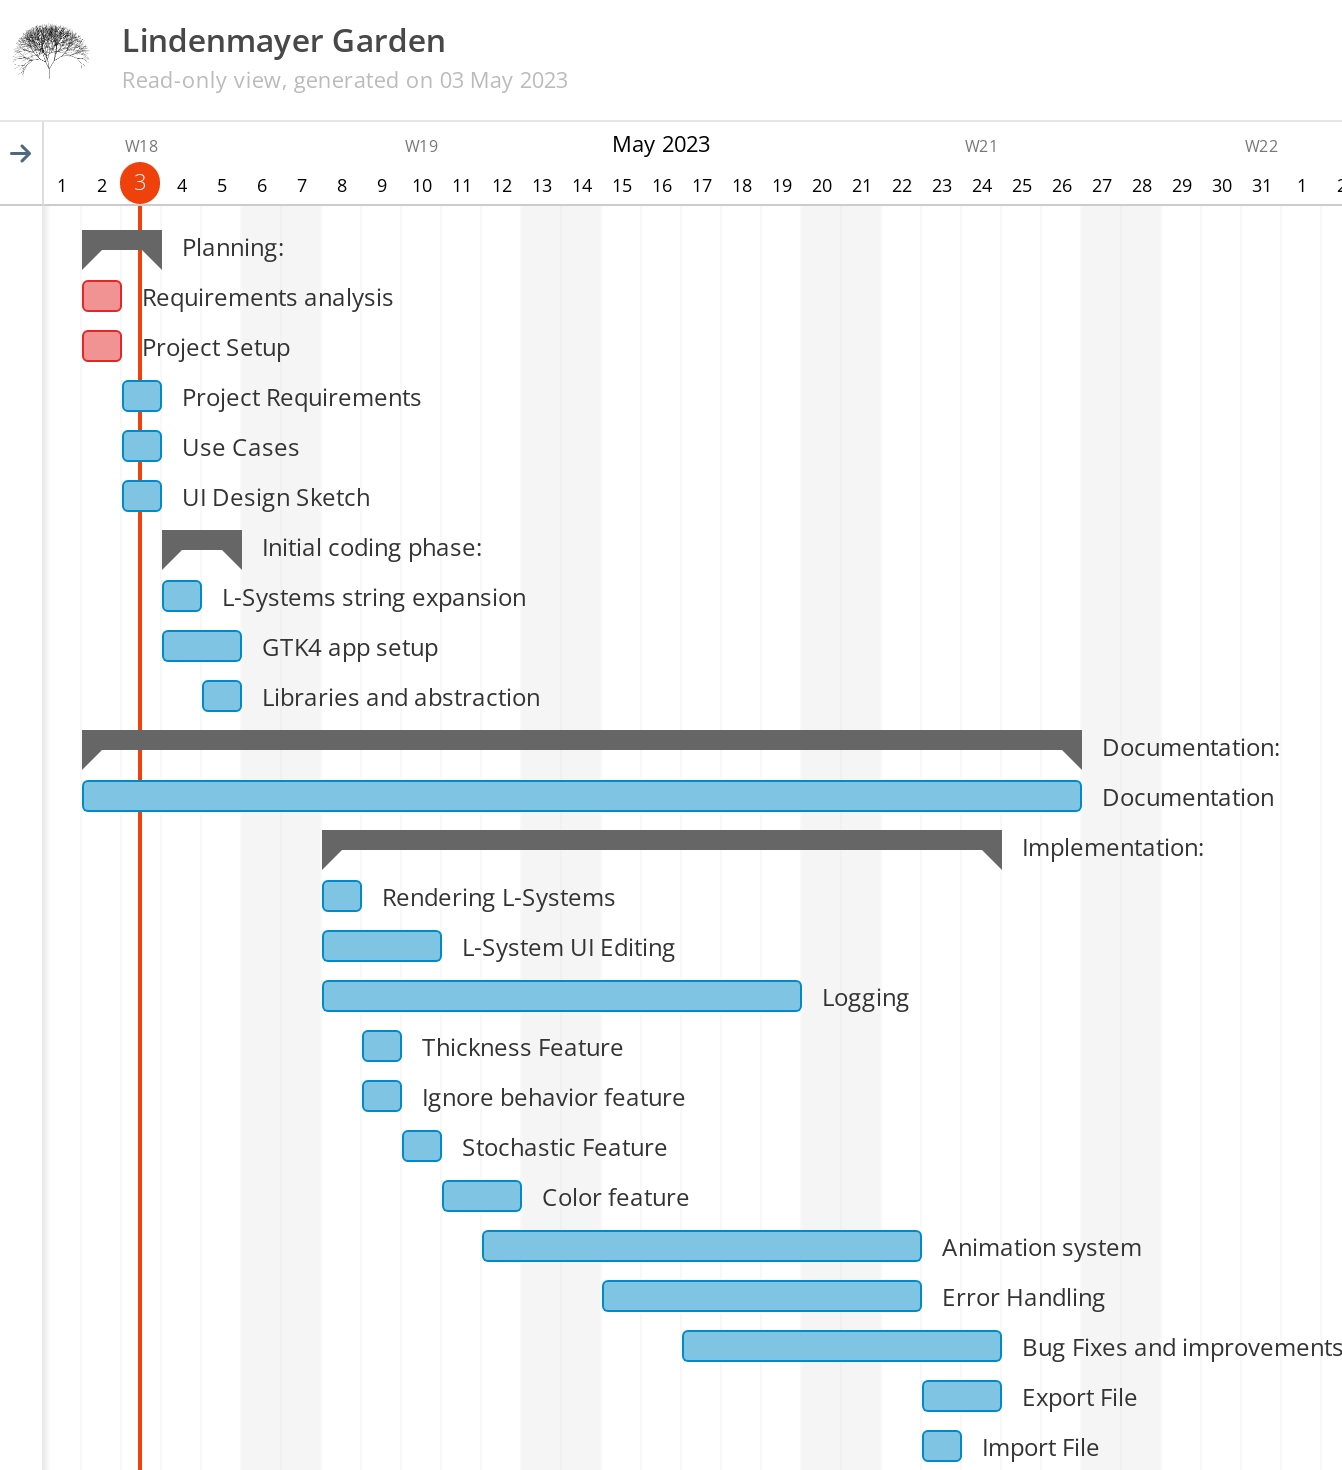
\includegraphics[width=\textwidth]{media/gantt/gantt1.jpg}
    \caption{Initial Gantt Chart}
\end{figure}

I chose the \gls{waterfall} model with a \Gls{Gantt} chart for my planning.

At the start of the project, I was pretty familiar with what I had to do
and how I was going to do it.
I tried to estimate the duration of the tasks based on this information.
I included a bit of margin towards the end to still have time to solve some eventual problems.

\pagebreak

\subsection{Final Gantt Chart}

% vesej19976@duscore.com
\begin{figure}[h]
    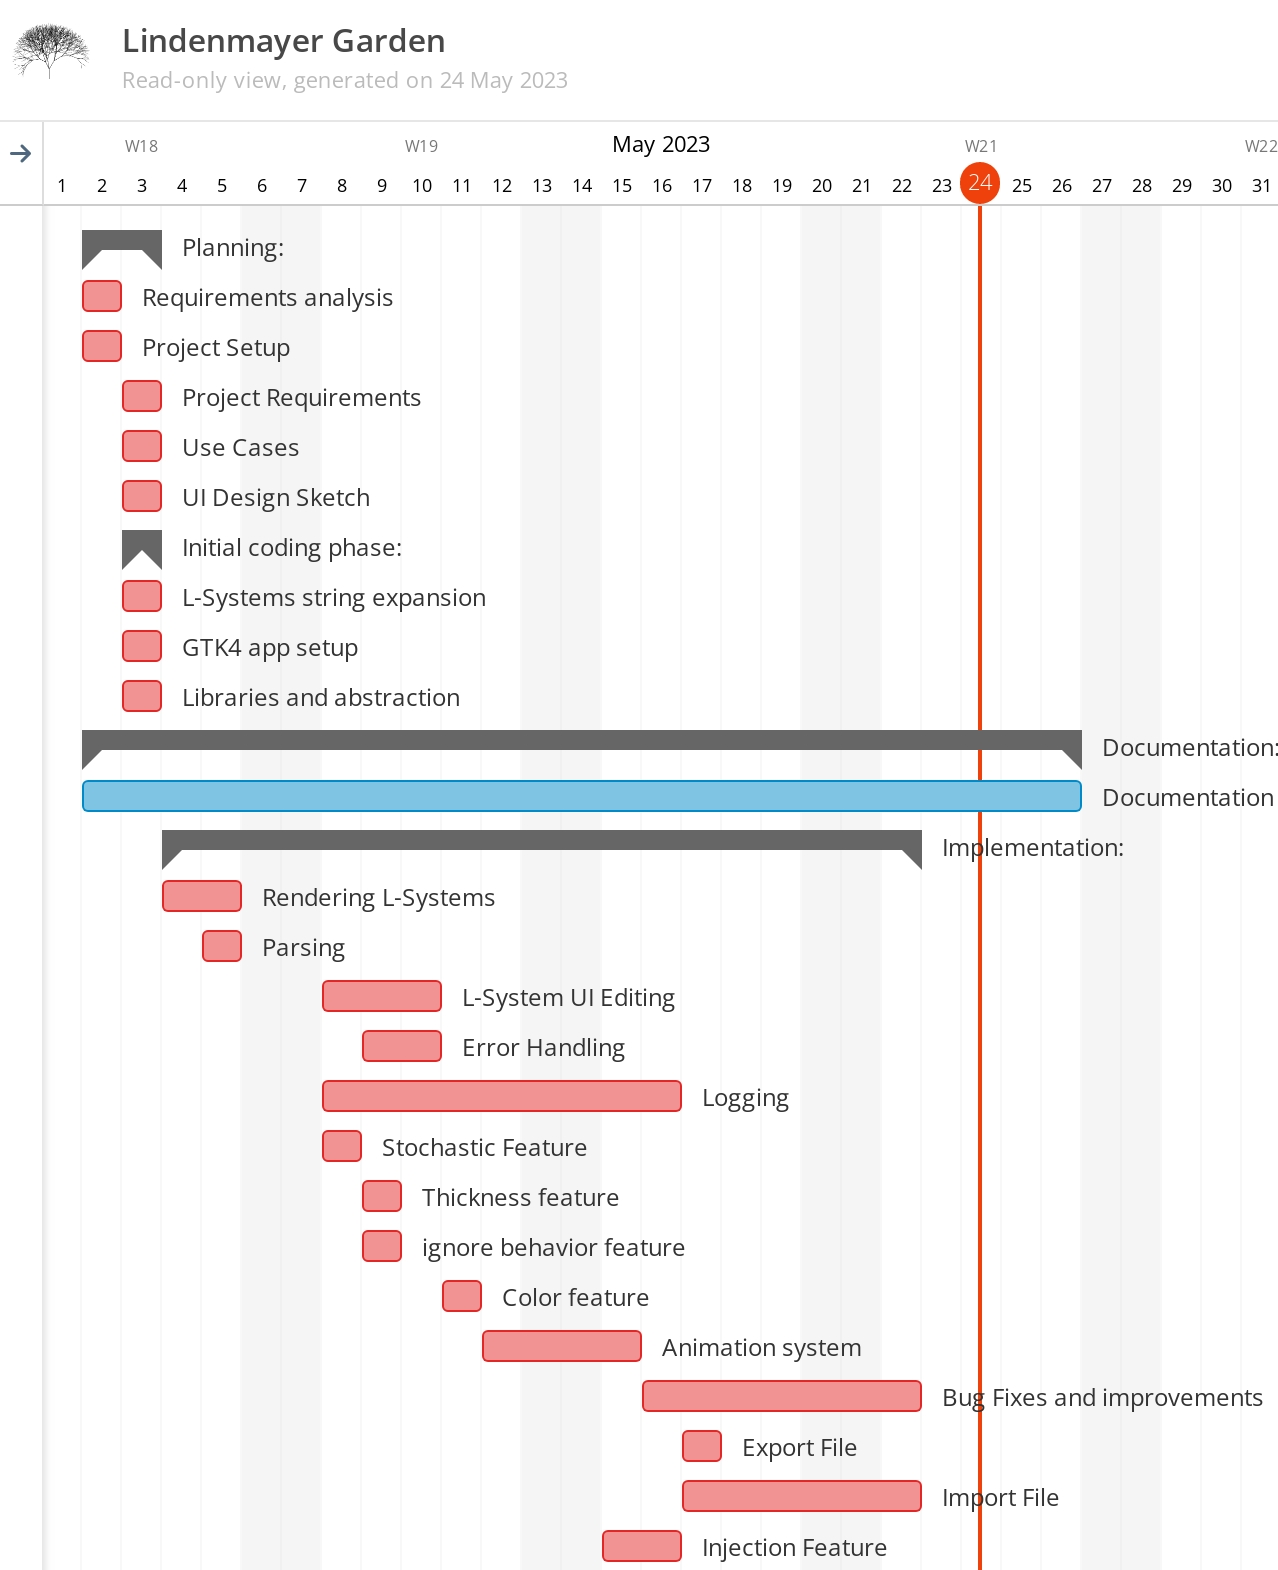
\includegraphics[width=\textwidth]{media/gantt/gantt2.jpg}
    \caption{Final Gantt Chart}
\end{figure}

I had a great start by completing early the whole \texttt{Initial Coding Phase}
section, which I had overestimated.
Thus, I was always 2-3 days early with respect to my initial planning.
\\
In general, almost every task was completed early.
The \texttt{Error Handling} task was done with the \texttt{UI Editing}.

Towards the end of the project, I spent much time implementing minor features and fixing bugs.
However, I still finished programming a couple of days early.

\pagebreak

\section{Compilation and usage}

In order to compile the application, you need to have GTK4 installed on your system.

\textbf{Using pacman}:
\begin{lstlisting}[style=boxed]
    $ pacman -S gtk4 base-devel
\end{lstlisting}

\textbf{Using dnf}:
\begin{lstlisting}[style=boxed]
    $ dnf install gtk4-devel gcc
\end{lstlisting}

\textbf{Using apt}:
\begin{lstlisting}[style=boxed]
    $ apt install libgtk-4-dev build-essential
\end{lstlisting}

For other platforms and information, visit this \href{https://gtk-rs.org/gtk4-rs/git/book/installation.html}{website}\cite{gtkinstallation}.

The executable can be compiled using the \texttt{\gls{cargo}}
package manager, which can be installed at the
\href{https://www.rust-lang.org/tools/install}{official website}\cite{rustinstall}.

\begin{lstlisting}[style=boxed]
    $ cd lindenmayer-gui
    $ cargo build --release
\end{lstlisting}

This will generate an executable (\texttt{lindenmayer-gui})
in \texttt{./target/release}.
In order to make this executable globally available,
you can move it into a folder in the \textsc{\$PATH} environment
variable, such as \texttt{/usr/bin}.
You may also modify the executable file name to change its invocation
name.

\begin{lstlisting}[style=boxed]
    $ sudo mv target/release/lindenmayer-gui /usr/bin/
\end{lstlisting}

The executable can now be invoked by just writing
\begin{lstlisting}[style=boxed]
    $ lindenmayer-gui
\end{lstlisting}

\pagebreak

\section{Implementation}

\subsection{Textual configuration}

The L-systems are represented by a textual configuration,
where each line indicates a property.
The conventional extension for this format is the \texttt{.lsys} extension.

There are four types of lines: 
\texttt{configurations},
\texttt{variables}, \texttt{operations} and \texttt{rules}.

\subsubsection{Sintax}

The configuration files have the following form.

\begin{lstlisting}[style=boxed]
[
    <Config>
    |
    <Variable>
    |
    <Operation>
    |
    <Rule>
]*
\end{lstlisting}

Different types of lines may be written in any order.

A \textbf{Configuration} element is defined as one of the following expressions:
\begin{lstlisting}[style=boxed]
    axiom <String>
    iter <Integer>
    initial_rot <Float>
    initial_pos <Position>
    initial_thickness <Float>
    initial_color <Color>
    background <Color>
    canvas <Dimension>
    seed <String>
    inject [<Injection>]*
\end{lstlisting}
If the same configuration command is repeated multiple times,
only the last one will be considered.

A \textbf{Variable} element is defined as
\begin{lstlisting}[style=boxed]
    VAR_NAME = <Number>
\end{lstlisting}

An \text{Operation} element is defined as one of the following expressions:
\begin{lstlisting}[style=boxed]
    <Char>: forward <Expression>
    <Char>: jump <Expression>
    <Char>: dot <Expression>
    <Char>: rotate <Expression>
    <Char>: thickness <Expression>
    <Char>: ignore <Expression>
    <Char>: push
    <Char>: pop
    <Char>: color <Color>
    <Char>: <Variable> = <Expression>
\end{lstlisting}

A \textbf{Rule} element is defined as
\begin{lstlisting}[style=boxed]
    <Char> -> <String>
\end{lstlisting}

%%%%%%%%%%%%% sub types

A \textbf{Position} element is defined as a tuple of floating point numbers
\begin{lstlisting}[style=boxed]
    Float,Float
\end{lstlisting}

A \textbf{Dimension} element is defined as a tuple of integers
\begin{lstlisting}[style=boxed]
    Integer,Integer
\end{lstlisting}

An \textbf{Injection} element is defined as a tuple of an integer (index) and a string (injection).
\begin{lstlisting}[style=boxed]
    Integer,String
\end{lstlisting}

A \textbf{Color} element is defined as a subset of strings that represent a valid color in the \gls{CSS} format\cite{csscolors}.

An \textbf{Expression} element is a \gls{CAS} (Computer Algebra System) expression.
The expression may use elementary functions and variables.
The expression may use the following functions
\begin{enumerate}
    \item \texttt{sqrt}: \(\sqrt{x}\). E.g. \texttt{sqrt(1)}.
    \item \texttt{exp}: \(e^x\). E.g. \texttt{exp(1)}.
    \item \texttt{ln}: \(\ln(x)\). E.g. \texttt{ln(1)}.
    \item \texttt{abs}: \(|x|\). E.g. \texttt{abs(1)}.
    
    \item \texttt{sin}: \(\sin(x)\). E.g. \texttt{sin(1)}.
    \item \texttt{cos}: \(\cos(x)\). E.g. \texttt{cos(1)}.
    \item \texttt{tan}: \(\tan(x)\). E.g. \texttt{tan(1)}.
    \item \texttt{asin}: \(\arcsin(x)\). E.g. \texttt{asin(1)}.
    \item \texttt{acos}: \(\arccos(x)\). E.g. \texttt{acos(1)}.
    \item \texttt{atan}: \(\arctan(x)\). E.g. \texttt{atan(1)}.
    \item \texttt{sinh}: \(\sinh(x)\). E.g. \texttt{sinh(1)}.
    \item \texttt{cosh}: \(\cosh(x)\). E.g. \texttt{cosh(1)}.
    \item \texttt{tanh}: \(\tanh(x)\). E.g. \texttt{tanh(1)}.
    \item \texttt{asinh}: \(\text{asinh}(x)\). E.g. \texttt{asinh(1)}.
    \item \texttt{acosh}: \(\text{acosh}(x)\). E.g. \texttt{acosh(1)}.
    \item \texttt{atanh}: \(\text{atanh}(x)\). E.g. \texttt{atanh(0.1)}.
    \item \texttt{floor}: \(\lfloor x \rfloor\). E.g. \texttt{floor(1)}.
    \item \texttt{ceil}: \(\lceil x \rceil\). E.g. \texttt{ceil(1)}.
    \item \texttt{round}: \(\text{round}(x)\). E.g. \texttt{round(1.1)}.
    \item \texttt{signum}: \(\text{sgn}(x)\). E.g. \texttt{signum(1)}.
    \item \texttt{atan2}: \(\text{atan2}(y,x)\). E.g. \texttt{atan2(10,1)}.
    \item \texttt{min}: \(\min(x_1, x_2, \cdots, x_n)\). E.g. \texttt{min(1, 10)}.
    \item \texttt{max}: \(\max(x_1, x_2, \cdots, x_n)\). E.g. \texttt{max(1, 10)}.
    \item \texttt{rand}: E.g. \texttt{rand(1, 10)}.
\end{enumerate}

\pagebreak

An expression may use variables in its syntax.
The available variables are the ones defined using variable expressions,
and a finite set of hard-coded values, namely:
\begin{enumerate}
    \item \texttt{pi}: \(\pi \approx 3.1415926\).
    \item \texttt{e}: \(e \approx 2.7182818\).
    \item \texttt{FRAME}: The current animation frame index.
    \item \texttt{TIME}: The elapsed time from the beginning of the animation.
    \item \texttt{INDEX}: The index of the symbol in the expanded fractal string that is being evaluated.
    \item \texttt{LENGTH}: The length of the expanded fractal string.
    \item \texttt{DEPTH}: The current stack depth.
\end{enumerate}

\pagebreak

\subsubsection{Examples}

The following shows an example of the \texttt{lsys} extension.

\begin{lstlisting}[style=boxed]
    axiom F
    iter 4
    initial_pos 400,820
    initial_rot 0
    initial_thickness 1
    background rgb(156, 198, 236)
    initial_color #006400ff
    canvas 750,800
    seed Windy Algae
    inject 5999,! 7500,!
    
    LINE = 10
    ANGLE = 0.36
    WIND_STRENGTH = 0.005
    SPEED = 0.005
    
    F: forward LINE
    +: rotate ANGLE + sin(SPEED*TIME*INDEX/LENGTH)*WIND_STRENGTH
    -: rotate -ANGLE
    [: push
    ]: pop
    !: ignore 1
    
    F -> FF+[+F-F-F]-[-F+F+F]
\end{lstlisting}

%\subsection{GTK}
%\subsection{Glib}
%\subsection{Cairo}

\subsection{Meval crate}

The meval crate\cite{meval} provides a simple math expression
parsing and evaluation. \\
It is able to parse and evaluate math expressions
with custom variables and functions. 

\begin{lstlisting}[style=Rust, style=boxed]
    use meval::{Expr, Context};

    let y = 1.;
    let expr: Expr = "phi(-2 * zeta + 1)".parse().unwrap();

    // Custom functions and variables
    let mut ctx = Context::new();
    ctx.func("phi", |x| x + y);
    ctx.var("zeta", -1.);

    let value = expr.eval_with_context(ctx).unwrap();
\end{lstlisting}

\subsection{Separation of concerns}

The application has been separated into
four crates and the main application.

The following commutative diagram shows the functional dependencies between the crates.
The arrow \(A \rightarrow B\) means \quotes{A depends on B}.

% dependencies
% https://q.uiver.app/#q=WzAsNSxbMSwxLCJcXHRleHR7Z3VpfSJdLFsyLDEsIlxcdGV4dHtwYXJzZXJ9Il0sWzEsMCwiXFx0ZXh0e3JlbmRlcmVyfSJdLFsyLDAsIlxcdGV4dHtlbmdpbmV9Il0sWzAsMCwiXFx0ZXh0e3JlbmRlcmVyLWNhaXJvfSJdLFswLDFdLFswLDJdLFswLDRdLFsxLDJdLFsyLDNdLFs0LDJdXQ==
\[\begin{tikzcd}
	{\text{renderer-cairo}} & {\text{renderer}} & {\text{engine}} \\
	& {\text{gui}} & {\text{parser}}
	\arrow[from=2-2, to=2-3]
	\arrow[from=2-2, to=1-2]
	\arrow[from=2-2, to=1-1]
	\arrow[from=2-3, to=1-2]
	\arrow[from=1-2, to=1-3]
	\arrow[from=1-1, to=1-2]
\end{tikzcd}\]

\subsubsection{lindenmayer-engine}

The purpose of this crate is to provide a basic
L-system interface capable of applying the rules
to a string.

This crate only handles the \texttt{axiom}
and the \texttt{rules}.

It exports the following struct

\begin{lstlisting}[style=Rust, style=boxed]
    #[derive(Debug)]
    pub struct LSystem {
        pub axiom: String,
        pub rules: HashMap<char, String>,
    }
    
    impl LSystem {
        pub fn new(axiom: &str, rules: &[(char, String)]) -> Self;

        // Expand from axiom
        pub fn expand(&self, iter: usize) -> String;
    
        // Expand any string
        pub fn apply_rules(&self, expression: String) -> String;
    }
\end{lstlisting}

\subsubsection{lindenmayer-renderer}

This crate is a wrapper around \texttt{lindenmayer\_engine::LSystem}
by handling all the rendering-related variables. \\
Its purpose is to handle the graphical meaning of each symbol
and represent variables and values.

This crate exports a drawing abstraction for a \texttt{Canvas}.

\begin{lstlisting}[style=Rust, style=boxed]
    pub trait Canvas {
        fn move_to(&self, x: f64, y: f64);

        fn line_to(&self, x: f64, y: f64);
    
        fn stroke(&self);
    
        fn save(&self);
    
        fn restore(&self);
    
        fn set_line_width(&self, thickness: f64);
    
        fn rectangle(&self, x: f64, y: f64, width: f64, height: f64);
    
        fn set_color(&self, r: f64, g: f64, b: f64, a: f64);
    
        fn arc(&self, x: f64, y: f64, r: f64);
    
        fn fill(&self);
    }
\end{lstlisting}

\pagebreak

The following shows the wrapper around \texttt{lindenmayer\_engine::LSystem}
along with the needed structures.

\begin{lstlisting}[style=Rust, style=boxed]
    #[derive(Debug)]
    pub enum Operation {
        Forward(Expr),
        Jump(Expr),
        Dot(Expr),
        Rotate(Expr),
        Thickness(Expr),
        Ignore(Expr),
        PushStack,
        PopStack,
        SetColor((f64, f64, f64, f64)),
        SetVar(String, Expr),
    }
    
    #[derive(Debug)]
    pub struct LSystemRenderer {
        pub lsystem: LSystem,
        pub iter: usize,
        pub initial_pos: (f64, f64),
        pub initial_rot: f64,
        pub initial_thickness: f64,
        pub background_color: (f64, f64, f64, f64),
        pub initial_color: (f64, f64, f64, f64),
        pub canvas: (i32, i32),
        pub seed: String,
        pub injections: Vec<(u32, String)>,
        pub variables: HashMap<String, f64>,
        pub operations: HashMap<char, Operation>,
        pub expression: String,
        pub rng: Rc<RefCell<Pcg64>>,
    }
    
    impl Default for LSystemRenderer;
    
    impl LSystemRenderer {
        pub fn new(
            pub lsystem: LSystem,
            pub iter: usize,
            pub initial_pos: (f64, f64),
            pub initial_rot: f64,
            pub initial_thickness: f64,
            pub background_color: (f64, f64, f64, f64),
            pub initial_color: (f64, f64, f64, f64),
            pub canvas: (i32, i32),
            pub seed: String,
            pub injections: Vec<(u32, String)>,
            pub variables: HashMap<String, f64>,
            pub operations: HashMap<char, Operation>,
            pub expression: String,
            pub rng: Rc<RefCell<Pcg64>>,
        ) -> Self;
    
        pub fn update_expr(&mut self);

        pub fn update_rng(&mut self);
    }
\end{lstlisting}

\pagebreak

Any structure implementing the \texttt{Canvas} \gls{trait}
has an implementation of the L-system rendering algorithm.

\begin{lstlisting}[style=Rust, style=boxed]
    impl dyn Canvas {
        pub fn draw_fractal<'a>(
            &self,
            fractal: &LSystemRenderer,
            variables: &'a mut ExprContext,
        ) -> Result<(), meval::Error>;
    } 
\end{lstlisting}

This implementation is responsible for the injection of all the \gls{CAS} functions
and the variables \texttt{DEPTH}, \texttt{INDEX}, \texttt{LENGTH}, \texttt{pi} and \texttt{e}.

\subsubsection{lindenmayer-renderer-cairo}

This crate is an implementation of the \texttt{lindenmayer\_renderer::Canvas}
\gls{trait} for the \texttt{cairo::Context} type.

\subsubsection{lindenmayer-parser}

This crate is an import and export layer for \texttt{lindenmayer\_renderer::LSystemRenderer}
using textual configuration.

This crate defines the syntax of the \texttt{lsys} file.

\subsubsection{lindenmayer-gui}

This project is an executable which starts the graphical user interface upon execution.

The \gls{GUI} adds a layer of abstraction to the renderer, which handles animations. \\
The hard-coded variables \texttt{TIME} and \texttt{FRAME} are indeed injected into the grammar
by the \gls{GUI} program.

\pagebreak

\subsection{Graphical User Interface}

The following image shows the application upon start. The editor is empty, thus a white canvas is rendered.

\begin{figure}[h]
    \centering
    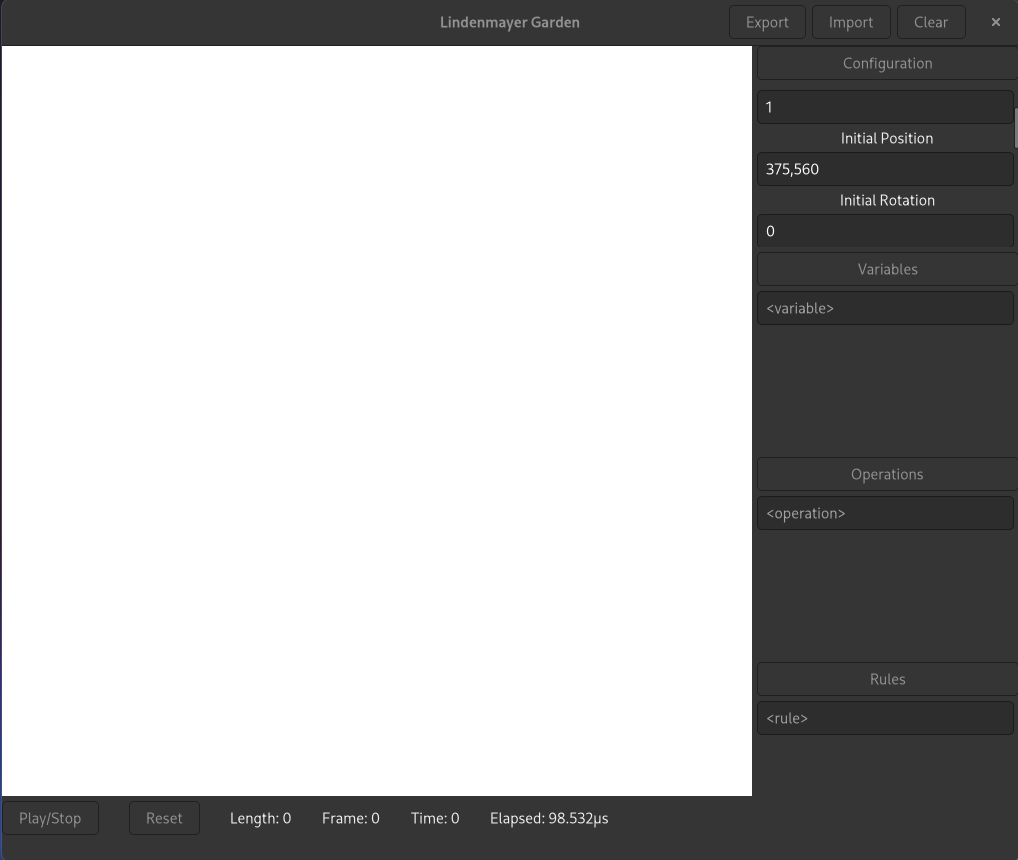
\includegraphics[width=0.8\textwidth]{media/gui/gui-empty.png}
    \label{fig:whitecanvas}
    \caption{Graphical User Interface - Empty}
\end{figure}

The graphical user interfaces is mainly composed of 3 sections:
\begin{itemize}
    \item A canvas where the fractal is rendered.
    \item A playback section to control the animation and display some properties about it.
    \item An editor section to edit the fractal in real-time according to the \texttt{lsys} format.
\end{itemize}

The editor section consists of four retractable subsections.
The subsections contain the \textit{configurations}, \textit{variables}, \textit{operations}
and \textit{rules} values respectively. \\
The latter 3 subsections are dynamic, meaning that entries are added or removed as needed.
The \textit{configurations} subsection is static. Every entry in this subsection is hard-coded
and the user is not required to prefix each value with its command.

\pagebreak

Here are more examples of the \gls{GUI} with different configurations

% windows are 1017x863

\begin{figure}[h]
    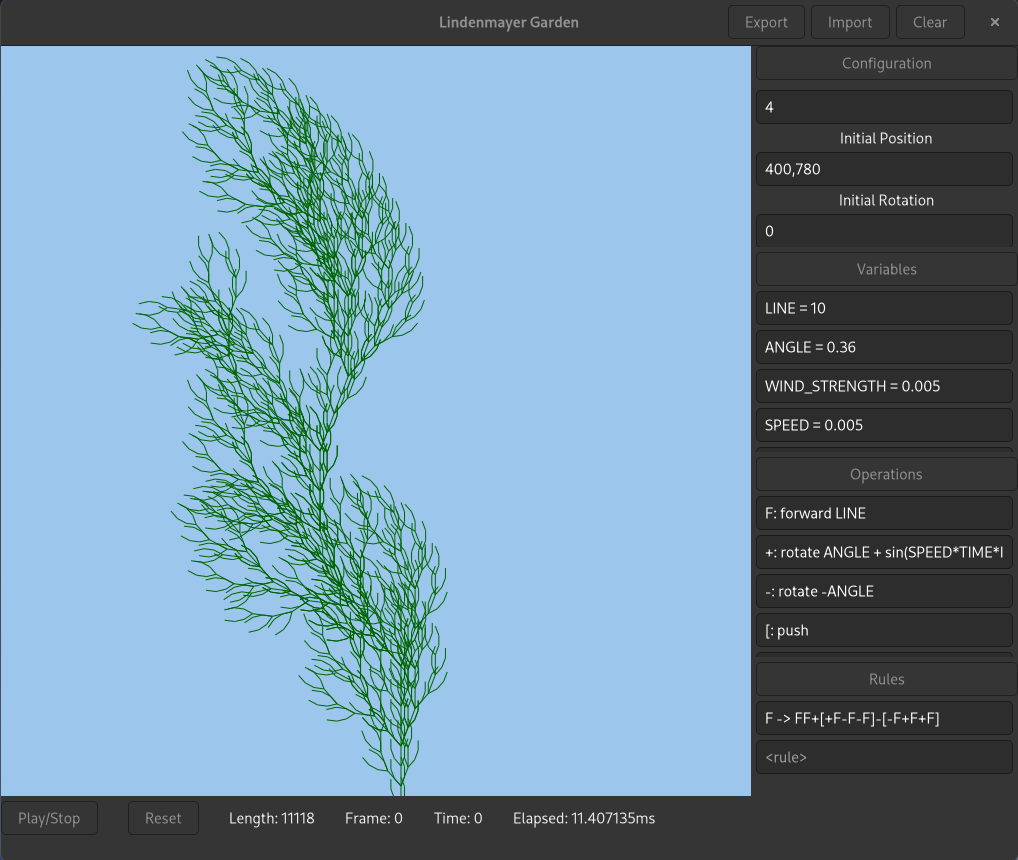
\includegraphics[width=\textwidth]{media/gui/gui-algae.png}
    \label{fig:algae}
    \caption{Algae Fractal}
\end{figure}

\begin{lstlisting}[style=boxed]
iter 4
initial_pos 400,820
background rgb(156, 198, 236)
initial_color #006400ff
canvas 750,800
inject 5999,! 7500,!

LINE = 10
ANGLE = 0.36
WIND_STRENGTH = 0.005
SPEED = 0.005

F: forward LINE
+: rotate ANGLE + sin(SPEED*TIME*INDEX/LENGTH)*WIND_STRENGTH
-: rotate -ANGLE
[: push
]: pop
!: ignore 1

F -> FF+[+F-F-F]-[-F+F+F]
\end{lstlisting}

\pagebreak
%%%%%%%%%%%%%%%%%%%%%%%%%

\begin{figure}[h]
    \centering
    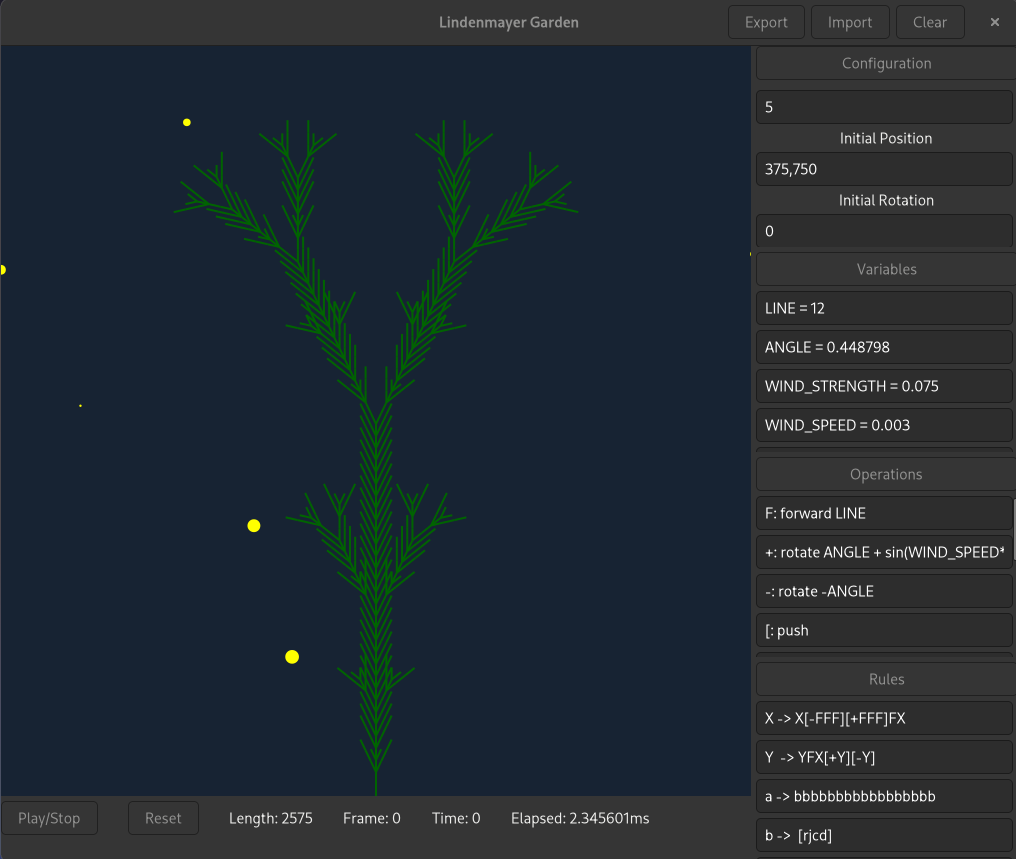
\includegraphics[width=0.9\textwidth]{media/gui/gui-fireflies.png}
    \label{fig:fireflies}
    \caption{Fireflies Fractal}
\end{figure}

\begin{lstlisting}[style=boxed]
axiom [Y]a
iter 5
initial_pos 375,750
initial_thickness 2
background #172333
initial_color #006400ff
canvas 750,750

LINE = 12
ANGLE = 0.448798
WIND_STRENGTH = 0.075
WIND_SPEED = 0.003

F: forward LINE 
+: rotate ANGLE + sin(WIND_SPEED*TIME*INDEX/LENGTH)*WIND_STRENGTH
-: rotate -ANGLE
[: push
]: pop
r: rotate pi*0.2*sin(INDEX) + 0.02*cos(FRAME*INDEX*0.000001)
j: jump 100+300*(1+sin(INDEX*51))+ 10*sin(TIME*INDEX*0.000001)
c: color yellow
d: dot 7*sin((100000 + TIME)*INDEX*0.000001)

X -> X[-FFF][+FFF]FX
Y -> YFX[+Y][-Y]
a -> bbbbbbbbbbbbbbbbb
b -> [rjcd]
\end{lstlisting}

\pagebreak
%%%%%%%%%%%%%%%%%%%%%%%%%

\begin{figure}[h]
    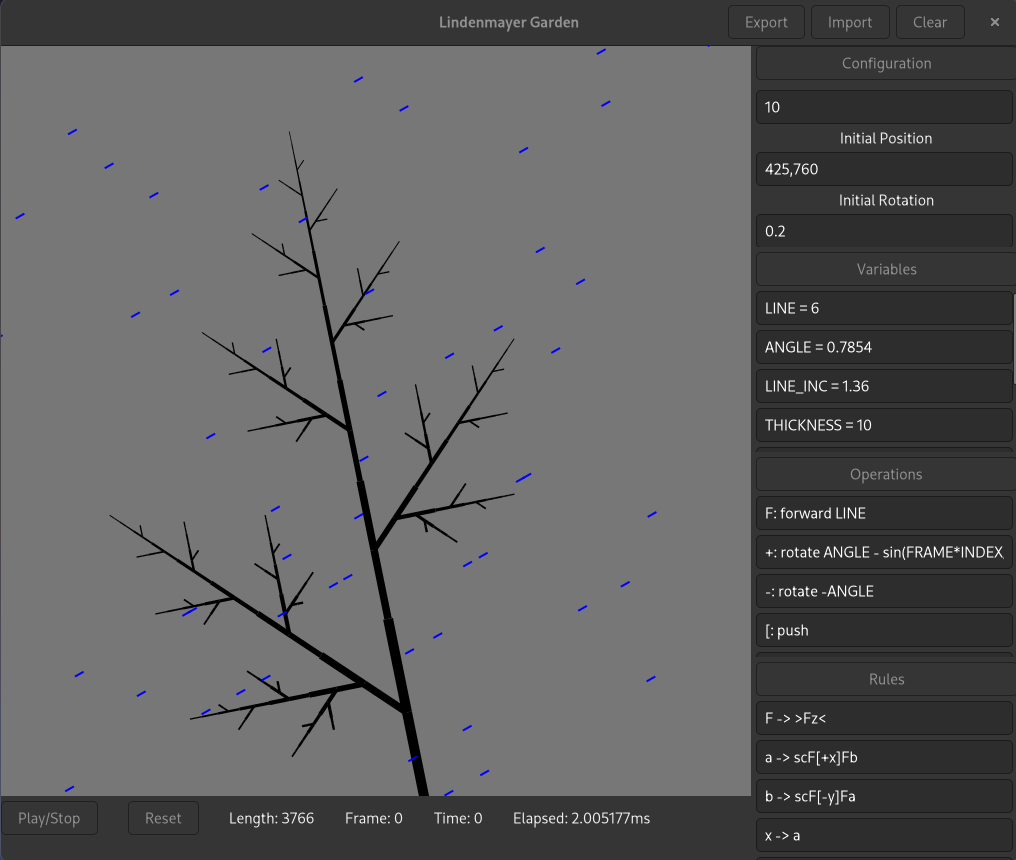
\includegraphics[width=\textwidth]{media/gui/gui-storm.png}
    \label{fig:storm}
    \caption{Storm Fractal}
\end{figure}

\begin{lstlisting}[style=boxed]
axiom [a]X
iter 10
initial_pos 425,760
initial_rot 0.2
background #777
initial_color #000000ff
canvas 750,750

LINE = 6
ANGLE = 0.7854
LINE_INC = 1.36
THICKNESS = 10
WIND_STRENGTH = 0.01
TURBULENCE = 0.2

F: forward LINE
+: rotate ANGLE - sin(FRAME*INDEX/LENGTH)/50
-: rotate -ANGLE
[: push
]: pop
>: LINE = LINE * LINE_INC
<: LINE = LINE / LINE_INC
s: thickness THICKNESS
c: THICKNESS = THICKNESS * 0.75
z: rotate abs(sin(TURBULENCE*FRAME*INDEX/LENGTH)*WIND_STRENGTH)
P: jump -400
V: rotate -pi*0.4
C: color blue
f: jump sin(INDEX)*500
J: jump 50
d: forward max(0, signum(sin((1000000+TIME)*INDEX*INDEX*0.000000002)))*10
T: thickness 2

F -> >Fz<
a -> scF[+x]Fb
b -> scF[-y]Fa
x -> a
y -> b
X -> TC[B]J[B]J[B]J[B]J[B]J[B]J[B]J[B]J[B]J[B]J[B]J[B]J[B]J[B]J[B]J[B]J[B]
B -> VPJDJDJDJDJDJDJDJDJDJDJDJDJDJDJ
D -> f[d]
\end{lstlisting}

\pagebreak

\subsection{Error Handling}

Whenever the editor notifies a change in any line, the whole configuration
is parsed from scratched. If there aren't any errors, the renderer is updated to render the new fractal.

The graphical user interface program extends the errors given by the parser
in order to signal an error if a \texttt{lsys} line is written in the wrong section.

The following image shows two correct \texttt{lsys} lines in the wrong section.
\begin{figure}[h]
    \centering
    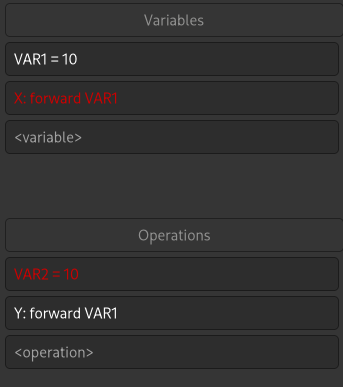
\includegraphics[width=0.5\textwidth]{media/gui/gui-err.png}
    \caption{Graphical User Interface - Error}
\end{figure}

\pagebreak

\subsection{Project Structure}

The following section shows the meaning of each file in the project source code.

\textbf{lindenmayer-engine}
\dirtree{%
.1 src.
.2 lib.rs | Exports the basic \texttt{LSystem} implementation (string expansion).
}

\textbf{lindenmayer-renderer}
\dirtree{%
.1 src.
.2 lib.rs | Exports \texttt{LSystemRenderer} structure.
.2 canvas.rs  | Contains the rendering implementation.
.2 expressions.
.3 mod.rs | Contains the \texttt{rand} functino.
}

\textbf{lindenmayer-renderer-cairo}
\dirtree{%
.1 src.
.2 lib.rs | Exports the drawing implementation.
}

\textbf{lindenmayer-parser}
\dirtree{%
.1 src.
.2 import.rs | Contains the import logic.
.2 export.rs | Contains the export logic.
.2 lib.rs | Module export.
}

\textbf{lindenmayer-gui}
\dirtree{%
.1 src.
.2 main.rs | Main program entry.
.2 ui.rs | Contains every element of the UI.
.2 logic.rs | Contains the main logic of the interactions between the UI and the backend.
.2 helpers.rs | Generic function helpers.
.2 config.rs | Utils to handle the configuration of the editor.
.2 animations.rs | Contains the animation logic layer.
.2 style.
.3 style.css | \gls{CSS} Styling of the UI.
}

\pagebreak

\subsection{Logging system}

The logging level and logging style can be set
by exporting the \colorbox{gray!10}{LSYS\_LOG} and \\
\colorbox{gray!10}{LSYS\_LOG\_STYLE}
environmental variables. The variables represent the log level
and the log style respectively.

The \colorbox{gray!10}{LSYS\_LOG} variable may assume the following values
\begin{itemize}
    \item \colorbox{gray!10}{error}: Designates very serious errors.
    \item \colorbox{gray!10}{warn}: Designates hazardous situations.
    \item \colorbox{gray!10}{info}: Designates useful information.
    \item \colorbox{gray!10}{debug}: Designates lower priority information.
    \item \colorbox{gray!10}{trace}: Designates very lower priority, often extremely verbose, information.
\end{itemize}
See \cite{envlogginglvl} for more information and more options.

The \colorbox{gray!10}{LSYS\_LOG\_STYLE} variable may assume the following values
\begin{itemize}
    \item \colorbox{gray!10}{auto}: Will attempt to print style characters if possible.
    \item \colorbox{gray!10}{always}: Will always print style characters.
    \item \colorbox{gray!10}{never}: Will never print style characters.
\end{itemize}
See \cite{envloggingstyle} for more information.

If the \colorbox{gray!10}{LSYS\_LOG} environmental variable is not set,
the default log value will be \texttt{info}.

\pagebreak

\subsection{Dependencies}

The following is a list of all the libraries used within the project
crates.

\bgroup{}
\def\arraystretch{1.5}
\begin{center}
    \begin{tabular}{ |p{2cm}|p{4cm}|p{1.5cm}|p{2cm}| }
        \hline
        \multicolumn{4}{|c|}{\textbf{Dependency table (lindenmayer-engine)}} \\
        \hline
        \textbf{Name} & \textbf{Description} & \textbf{Version} & \textbf{Features} \\
        \hline
    \end{tabular}
\end{center}
\egroup{}

\bgroup{}
\def\arraystretch{1.5}
\begin{center}
    \begin{tabular}{ |p{2cm}|p{4cm}|p{1.5cm}|p{2cm}| }
        \hline
        \multicolumn{4}{|c|}{\textbf{Dependency table (lindenmayer-renderer)}} \\
        \hline
        \textbf{Name} & \textbf{Description} & \textbf{Version} & \textbf{Features} \\
        \hline
        meval & \gls{CAS} expressions parsing & 0.2.0 & \- \\
        \hline
        lindenmayer-engine & Basic L-system expansion & (local) & \- \\
        \hline
    \end{tabular}
\end{center}
\egroup{}

\bgroup{}
\def\arraystretch{1.5}
\begin{center}
    \begin{tabular}{ |p{2cm}|p{4cm}|p{1.5cm}|p{2cm}| }
        \hline
        \multicolumn{4}{|c|}{\textbf{Dependency table (lindenmayer-renderer-cairo)}} \\
        \hline
        \textbf{Name} & \textbf{Description} & \textbf{Version} & \textbf{Features} \\
        \hline
        cairo-rs & Cairo bindings & 0.17.0 & \- \\
        \hline
        lindenmayer-renderer & Rendering abstraction & (local) & \- \\
        \hline
    \end{tabular}
\end{center}
\egroup{}

\bgroup{}
\def\arraystretch{1.5}
\begin{center}
    \begin{tabular}{ |p{2cm}|p{4cm}|p{1.5cm}|p{2cm}| }
        \hline
        \multicolumn{4}{|c|}{\textbf{Dependency table (lindenmayer-parser)}} \\
        \hline
        \textbf{Name} & \textbf{Description} & \textbf{Version} & \textbf{Features} \\
        \hline
        csscolorparser & \gls{CSS} color parsing & 0.6.2 & \- \\
        \hline
        lindenmayer-renderer & Rendering abstraction & (local) & \- \\
        \hline
    \end{tabular}
\end{center}
\egroup{}

\bgroup{}
\def\arraystretch{1.5}
\begin{center}
    \begin{tabular}{ |p{2cm}|p{4cm}|p{1.5cm}|p{2cm}| }
        \hline
        \multicolumn{4}{|c|}{\textbf{Dependency table (lindenmayer-gui)}} \\
        \hline
        \textbf{Name} & \textbf{Description} & \textbf{Version} & \textbf{Features} \\
        \hline
        gtk & GTK4 & 0.6.0 & v4\_10 \\
        \hline
        cairo-rs & Cairo bindings & 0.17.0 & \- \\
        \hline
        log & Logging abstraction & 0.4.17 & \- \\
        \hline
        env\_logger & Logging implementation & 0.10.0 & \- \\
        \hline
        lindenmayer-renderer & Rendering abstraction & (local) & \- \\
        \hline
        lindenmayer-renderer-cairo & Drawing implementation & (local) & \- \\
        \hline
        lindenmayer-parsing & \texttt{lsys} format parsing & (local) & \- \\
        \hline
    \end{tabular}
\end{center}
\egroup{}

\pagebreak

\section{Tips and tricks}

\subsection{Random values}

The \texttt{rand(min, max)} function is pretty useless when designing an animation.
Animations cannot generally be smooth when using this function, as whatever value we are randomizing
will drastically change between frames, unless the range is very small. \\
To achieve the same result but keeping the same random values between frames,
I found the following method better: setup a variable \texttt{SEED = 42} and then use
the expression \texttt{sin(SEED + INDEX * INDEX)}. This provides a pseudo-random function
persistent between frames but different in each point of the fractal.
If you want a pseudo-random function persistent in every point of the fractal but different
between frames you can use \texttt{sin(SEED + FRAME * FRAME)} or \texttt{sin(SEED + TIME * TIME)}.

\subsection{Natural growth}

When designing a natural shaped tree, the symmetry of the fractal can be broken
to achieve a more natural growth. This can be achieved by injecting
symbols into the fractal string at arbitrary positions.
A common choice is the symbol \texttt{!: ignore 1}.
Alternatively, using the symbol \texttt{!: rand(0, 1.005)} in the production rules may also yield good results.

\subsection{Stochastic grammar}

It is possible to simulate the behavior of a stochastic context-free grammar
in a deterministic context-free grammar. \\
Let's define \texttt{X: forward 10} and \texttt{Y: dot 10}.
We want to define a rule such that the symbol \texttt{F} has a certain probability of becoming \texttt{X}
or \texttt{Y}.

Set up the following variables: \texttt{PROB = 0.5} (50\%) and \texttt{MEMORY = 0}. \\
Redefine \texttt{X} as \texttt{X: forward 10*MEMORY} and \texttt{Y} as \texttt{Y: dot 10*(1-MEMORY)}. \\
Let \texttt{M: MEMORY = max(0, signum((rand(0, 1)-PROB)))}. \\
The production rule is now \texttt{F -> MXY}.

The core idea is to always execute both \texttt{X} and \texttt{Y}, but make their values null in a mutually exclusive way.
The expression \texttt{max(0, signum((rand(0, 1)-PROB)))} is a distribution of \(0\) and \(1\) according
to the probability \texttt{PROB}.

\pagebreak

\section{Tests}

\subsection{Testing protocol}

\paragraph{Requirements:}
The following tests must satisfy the following requirements.
The resources can be found in the project source code.
Tests must be executed in order.

\begin{enumerate}
    \item The compiled executable of the \texttt{lindenmayer-gui} software
    must be placed in a folder specified in the \textsc{PATH}
    environmental variable (e.g. \texttt{/usr/local/bin} or \texttt{/usr/bin}).
    \item The \texttt{lindenmayer-gui} file must be an executable. It should be enough to run
    \lstinline{chmod +x <file>}.
    \item The user from which the tests will be executed must have permission to execute
    the program.
    \item The project examples must be available in the file system.
    \item The user must have the permission to read each resource used and write files
    to the specified locations.
    \item Some compositors do not render the buttons on the header bar of the application whilst in full screen mode.
    To avoid any problem, do not put the application in full screen mode.
    \item A text editor.
\end{enumerate}

\lstdefinestyle{logging} {
    basicstyle=\ttfamily,
    numbers=none,
    breaklines=true,
    backgroundcolor=\color[gray]{0.97},
    morekeywords={INFO},
    keywordstyle=\color[rgb]{0, 0.75, 0},
    morekeywords=[2]{ERROR},
    keywordstyle=[2]\color[rgb]{0.75, 0, 0},
    morekeywords=[3]{WARN},
    keywordstyle=[3]\color[rgb]{1, 0.5, 0},
    morekeywords=[4]{DEBUG},
    keywordstyle=[4]\color[rgb]{0.1, 0.1, 0.9}
}

\newcommand{\moveabit}[1]{\adjustbox{lap={\width}{-0.9cm}}{#1}}

\paragraph{Tests:}

\test{00}{Application Start}{Req-04}{
    \item Start the application by launching the \texttt{lindenmayer-gui} command.
}{%
    A window must appear on the screen with the same look and UI elements
    as the image (\ref{fig:whitecanvas}).
}

\test{01}{Initial error state}{Req-04, Req-06}{
    \item Focus on the \textit{Axiom} entry under the \textit{Configuration} section.
}{%
    The entry must glow red as it is the only error in the default configuration.
}

\test{02}{Dynamic entries 1}{\-}{
    \item Start the application by launching the \texttt{lindenmayer-gui} command.
    \item For each section (\texttt{Variables}, \texttt{Operations} and \texttt{Rules})
    start typing in the only available entry.
}{%
    A second entry must appear right beneath the first one.
}

\test{03}{Dynamic entries 2}{\-}{
    \item Delete the text written in the previous test from the entry
    of each section.
}{%
    The second entry must disappear.
}

\test{04}{Logging 1}{Req-05}{
    \item Start the application by launching the \texttt{lindenmayer-gui command}.
}{%
\makecell[tl]{
The output written to the \textsc{stdout} must look like this: \\
\begin{lstlisting}[style=logging]^^J
    [<time> INFO  lindenmayer_gui] Initializing application^^J
    [<time> INFO  lindenmayer_gui] Loading CSS stylesheet^^J
    [<time> INFO  lindenmayer_gui::logic] Initializing UI content^^J
    [<time> INFO  lindenmayer_gui::ui] Building UI^^J
    [<time> INFO  lindenmayer_gui::logic] Initializing configuration^^J
    [<time> WARN  lindenmayer_gui::helpers] Input is incorrect^^J
\end{lstlisting}
}
}

\test{05}{Logging 2}{Req-05}{
    \item \makecell[tl]{Start the application by launching the \\ \texttt{LSYS\_LOG=debug lindenmayer-gui} command.}
}{%
\makecell[tl]{
The output written to the \textsc{stdout} must look like this: \\
\begin{lstlisting}[style=logging]^^J
    [2023-05-24T07:50:18Z INFO  lindenmayer_gui] Initializing application^^J
    [2023-05-24T07:50:18Z INFO  lindenmayer_gui] Loading CSS stylesheet^^J
    [2023-05-24T07:50:18Z INFO  lindenmayer_gui::logic] Initializing UI content^^J
    [2023-05-24T07:50:18Z INFO  lindenmayer_gui::ui] Building UI^^J
    [2023-05-24T07:50:18Z INFO  lindenmayer_gui::logic] Initializing configuration^^J
    [2023-05-24T07:50:18Z WARN  lindenmayer_gui::helpers] Input is incorrect^^J
    [2023-05-24T07:50:18Z DEBUG lindenmayer_gui::animations] Updating renderer. Generating fractal^^J
    [2023-05-24T07:50:18Z DEBUG lindenmayer_gui::animations] String expansion took: 803ns^^J
\end{lstlisting}
}
}

\test{06}{Import feature}{Req-00, Req-01, Req-04}{
    \item Press the \texttt{Import} button at the top of the \gls{GUI}.
    \item Navigate to the examples folder and select the \texttt{fireflies.lsys} file.
    \item Press \texttt{Open}.
}{%
    A fractal must be rendered onto the canvas as in image (\ref{fig:fireflies}).
}

\test{07}{Real time editor}{Req-04, Req-00}{
    \item Under the \textit{Variables} section, focus on the \texttt{LINE} variable entry.
    \item Modify the text from \texttt{LINE = 12} to \texttt{LINE = 6}.
}{%
    The fractal must shrink to half its original size as soon as the text has been modified.
}

\test{08}{Export feature}{Req-04}{
    \item Press the \texttt{Export} button at the top of the \gls{GUI}.
    \item Save the file to the examples location with the name \texttt{fireflies2.lsys}.
    \item Press \texttt{Save}.
}{%
    Open the saved file with a text editor. The file must contain some data
    and the correct \texttt{LINE = 6} line.
}

\test{09}{Consistency}{Req-00, Req-01, Req-04}{
    \item Press the \texttt{Import} button at the top of the \gls{GUI}.
    \item Navigate to the examples folder and select the \texttt{fireflies2.lsys} file.
    \item Press \texttt{Open}.
}{%
    The same smaller fractal must be rendered onto the canvas.
}

\test{10}{Animation start}{Req-01, Req-03, Req-04}{
    \item Press the \texttt{Import} button at the top of the \gls{GUI}.
    \item Navigate to the examples folder and select the \texttt{algae.lsys} file.
    \item Press \texttt{Open}.
    \item Press the \texttt{Play/Stop} button under the canvas. 
}{%
    An animation must begin where the algae softly sways around.
}

\test{11}{Reset feature}{Req-04}{
    \item Press the \texttt{Reset} button under the canvas.
}{%
    The animation must restart from the beginning. The \texttt{Frame}
    and \texttt{Time} label under the canvas must restart from a value of \(0\).
}

\test{12}{Animation stop}{Req-03}{
    \item Press the \texttt{Play/Stop} button under the canvas multiple times.
}{%
    The animation must stop and resume at every other press of the button.
}

\test{13}{Clear feature}{Req-03, Req-04}{
    \item Press the \texttt{Clear} button at the top of the \gls{GUI}.
}{%
    The entire \gls{GUI} must be reset to its initial state of a white canvas and empty editor.
}

\test{14}{Retractable section}{Req-04}{
    \item Click on the titles of each of the four section.
}{%
    All the sections must hide their contents.
}

\test{15}{Syntax errors 1}{Req-01, Req-06}{
    \item Start the application by launching the \texttt{lindenmayer-gui} command.
    \item Press the \texttt{Import} button at the top of the GUI.
    \item Navigate to the examples folder and select the \texttt{storm.lsys} file.
    \item Press \texttt{Open}.
    \item Under the \textit{Operations} section, focus on the \texttt{F: forward LINE} entry.
    \item Modify the text from \texttt{F: forward LINE} to \texttt{F: hello LINE}.
}{%
    The entry must glow red as the operation is invalid.
}

\test{16}{Syntax errors 2}{Req-06}{
    \item Modify the text from \texttt{F: hello LINE} to \texttt{F: forward LINE}.
}{%
    The entry must stop glowing red as the operation is now valid again.
}

\test{17}{State errors}{Req-06}{
    \item Modify the text from \texttt{F: forward LINE} to \texttt{F: forward line}.
}{%
    A red label at the top of the editor must appear with the text: {\color{red}Invalid var: line}.
}

\test{18}{Stochastic behavior}{Req-02}{
    \item Modify the text from \texttt{F: forward line} to \texttt{F: forward LINE}.
    \item Under the \textit{Operations} section, focus on the \texttt{-: rotate -ANGLE} entry.
    \item Modify the text from \texttt{-: rotate -ANGLE} to \texttt{-: rotate rand(0,1)}.
}{%
    All the branches of the tree that were on the right side must now be on the left side
    at random angles
}

\test{19}{Random seed}{Req-02}{
    \item Under the \textit{Configuration} section, focus on the \texttt{seed} entry.
    \item Continuously add letters to the seed.
}{%
    As the seed changes, the branches of the tree at random angles must change their angle.
}

\pagebreak

\subsection{Test results}

Every test has successfully been passed.
The application still has some minor bugs, but it is stable.

\definecolor{darkgreen}{rgb}{0, 0.6, 0.2}
\bgroup{}
\def\arraystretch{1.25}
\begin{center}
    \begin{tabular}{ |l|l|l| }
        \hline
        \textbf{ID} & \textbf{Result} & \textbf{Note} \\
        \hline
        \textbf{Test-00} & \color{darkgreen} Passed & The application starts correctly. \\
        \hline
        \textbf{Test-01} & \color{darkgreen} Passed & The entry becomes red. \\
        \hline
        \textbf{Test-02} & \color{darkgreen} Passed & New entries are generated. \\
        \hline
        \textbf{Test-03} & \color{darkgreen} Passed & Entries are removed. \\
        \hline
        \textbf{Test-04} & \color{darkgreen} Passed & The output looks like the given one. \\
        \hline
        \textbf{Test-05} & \color{darkgreen} Passed & The output looks like the given one. \\
        \hline
        \textbf{Test-06} & \color{darkgreen} Passed & The fractal is rendered correctly. \\
        \hline
        \textbf{Test-07} & \color{darkgreen} Passed & The fractal shrinks its size. \\
        \hline
        \textbf{Test-08} & \color{darkgreen} Passed & The file contains the correct information. \\
        \hline
        \textbf{Test-09} & \color{darkgreen} Passed & The fractal is rendered correctly. \\
        \hline
        \textbf{Test-10} & \color{darkgreen} Passed & The animation plays correctly. \\
        \hline
        \textbf{Test-11} & \color{darkgreen} Passed & The animation restarts. \\
        \hline
        \textbf{Test-12} & \color{darkgreen} Passed & The animation stops. \\
        \hline
        \textbf{Test-13} & \color{darkgreen} Passed & The editor and canvas are cleared. \\
        \hline
        \textbf{Test-14} & \color{darkgreen} Passed & The sections retract correctly. \\
        \hline
        \textbf{Test-15} & \color{darkgreen} Passed & The entry glows red. \\
        \hline
        \textbf{Test-16} & \color{darkgreen} Passed & The entry stops glowing red. \\
        \hline
        \textbf{Test-17} & \color{darkgreen} Passed & The correct label appears. \\
        \hline
        \textbf{Test-18} & \color{darkgreen} Passed & The fractal changes accordingly. \\
        \hline
        \textbf{Test-19} & \color{darkgreen} Passed & The branches angles change randomly. \\
        \hline
    \end{tabular}
\end{center}
\egroup{}

\pagebreak

\section{Conclusions}

\subsection{Future development}

There are lots of features that could be added to the application
and improvements that could be made.
There are also some known bugs.

\begin{enumerate}
    \item \textbf{More features}: Additional drawing features could be added to the grammar
    of the system, such as polygons, line types, curves, functions and so on.
    \item \textbf{Parallel rendering}: The drawings are rendered by the main graphical thread.
    This results in the UI being slow if the rendering of the animation is particularly hard.
    \item \textbf{Resources exhaustion}: The string expansion of the fractal is done by the main graphical thread.
    If the user, for instance, accidentally adds a digit to the number of iterations, the program
    will start expanding the fractal string even if there is not enough RAM in the entire world
    that could contain it, resulting in the hard crash of the program.
    It would be useful to add a threshold within which the program will stop computing the fractal string,
    or a \quotes{safety mode} that can be activated/deactivated.
    \item \textbf{Refactor}: The overall structure of the code is, in my opinion, pretty good and flexible.
    However, if I could go back, I would definitly make it even better. The program relies too much on the
    \quotes{text format parsing}. Every time a value is changed in the editor, everything is parsed again from scratch.
    \item \textbf{Import/Export crash}: Sometimes the import and export features will crash whilst opening a folder in the file dialog.
    The error is caused by a \texttt{free(*ptr)} operation in the underlying libraries, but I have no idea how to fix it or
    if I even did something wrong, it may just be a library bug.
    \item \textbf{Stop rendering if error}: If the configuration is correct, but an expression uses an invalid variable or function,
    the render loop will keep going even thought nothing will be rendered.
    \item \textbf{Export}: An export feature of the render could be added. The program could export
    single frames as images, or record a part of an animation and export it as a video.
    \item \textbf{Grammar types}: It would be useful to support other grammar types, such as context-sensitive
    grammars or stochastic grammars.
    \item \textbf{Multiple operations}: Being able to associate multiple operations to a symbol \\
    (E.g. \texttt{F: ; rotate 0.1}) would drastically reduce the complexity of some systems.
    \item \textbf{Multiple renders bug}: If the canvas is not wide enough, such that the labels
    beneath it are larger than the canvas, the rendering of the frame will change the value in the \texttt{Elapsed}
    label. Since the labels occupy more space than the canvas, and the size of the \texttt{Elapsed} label changes,
    the left side of the UI changes its width, triggering another render operation to be called (and so on).
\end{enumerate}

\subsection{Personal conclusions}

The topic of the project was one of the best ones I had ever worked on.
I really enjoyed implementing new features, and I spent hours playing
with my own product.
I am very glad to have been able to shape the workings of the L-systems with my ideas,
which have extended the product beyond the requirements of the project.
I had many problems handling the memory within the \gls{GTK} application,
but in the end it all worked out, and
I learned much about memory management in \gls{Rust} and smart pointers.

\pagebreak

\begin{center}
    \thispagestyle{empty}
    \vspace*{\fill}
    \textsl{A picture of the Mandelbrot Set\cite{mandelbrot}
    drawn using an L-system.}
    \begin{figure}[h]
        \centering
        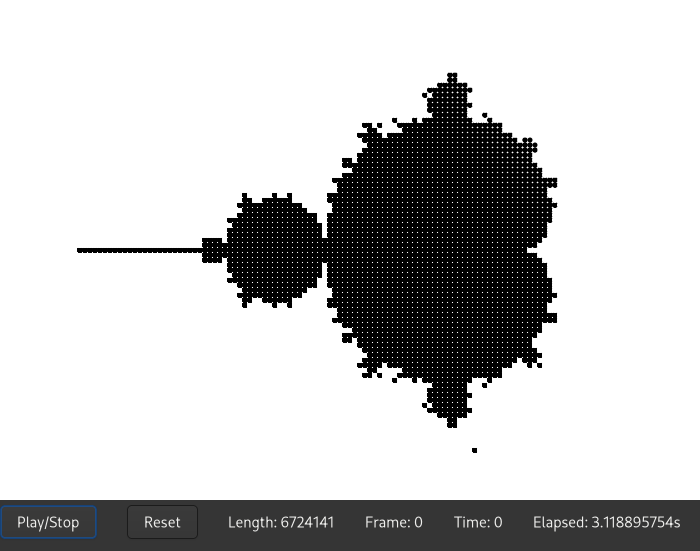
\includegraphics[width=0.75\textwidth]{media/gui/gui-mandelbrot.png}
        \caption{The Mandelbrot Set}
    \end{figure}
    \vspace*{\fill}
\end{center}

\pagebreak

\listoffigures

\pagebreak

\nocite{*} % cite all entries

\printbibliography

\pagebreak

\printnoidxglossary

\end{document}